{\documentclass[sigplan, screen]{acmart}
\usepackage[german, main=ngerman]{babel}
\usepackage{fancyhdr}
\usepackage{listings, lstautogobble}
\usepackage{tablefootnote}

\def\sectionautorefname{Abschnitt}
\def\subsectionautorefname{Abschnitt}
\def\subsubsectionautorefname{Abschnitt}
\def\tableautorefname{Tabelle}
\def\figureautorefname{Figur}
\def\lstlistingautorefname{Listing}

\AtBeginDocument{%
  \providecommand\BibTeX{{%
    \normalfont B\kern-0.5em{\scshape i\kern-0.25em b}\kern-0.8em\TeX}}}

\definecolor{backcolour}{rgb}{0.95,0.95,0.92}
\definecolor{lightgray}{rgb}{.9,.9,.9}
\definecolor{darkgray}{rgb}{.4,.4,.4}
\definecolor{purple}{rgb}{0.65, 0.12, 0.82}
\definecolor{lightgreen}{rgb}{0.45, 0.8, 0.45}

\lstdefinelanguage{JavaScript}{
  keywords={break, case, catch, continue, debugger, default, delete, do, else, false, finally, for, function, if, in, instanceof, new, null, return, switch, this, throw, true, try, typeof, var, void, while, with},
  keywordstyle=\color{purple}\bfseries,
  ndkeywords={type, class, export, boolean, throw, implements, import, this},
  ndkeywordstyle=\color{darkgray}\bfseries,
  identifierstyle=\color{black},
  sensitive=false,
  comment=[l]{//},
  morecomment=[s]{/*}{*/},
  commentstyle=\color{gray}\ttfamily,
  stringstyle=\color{lightgreen}\ttfamily,
  morestring=[b]',
  morestring=[b]"
}

\lstdefinestyle{mystyle}{
  language=JavaScript,
  basicstyle=\ttfamily\footnotesize,
  breakatwhitespace=false,         
  breaklines=true,                     
  keepspaces=true,                 
  numbers=left,                    
  numbersep=5pt,                  
  showspaces=false,                
  showstringspaces=false,
  showtabs=false,                  
  tabsize=2,
  autogobble=true,
  frame=single,
  columns=flexible
}

\lstset{style=mystyle}

\makeatletter
\newlength{\singlespace}
\newlength{\gobble}
\newlength{\numbersep}
% The width of a single space.
\settowidth{\singlespace}{\lst@basicstyle \ }
\setlength{\singlespace}{-\singlespace}

\lst@Key{firstlineandnumber}\relax{\def\lst@firstline{#1\relax}\def\lst@firstnumber{#1\relax}}
\makeatother

\setcopyright{none}
\settopmatter{printacmref=false, printfolios=true}
\renewcommand\footnotetextcopyrightpermission[1]{}
\copyrightyear{2022}
\acmYear{2022}

\acmBooktitle{Hauptseminar II WiSe 22/23, gehalten von Kevin Linne, M.Sc.}

\begin{document}

\title{Möglichkeiten zur asynchronen Kommunikation zwischen Webbrowser und Server}

\author{Hendrik Wagner}
\email{hendrik.wagner@mni.thm.de}

\affiliation{%
  \institution{Technische Hochschule Mittelhessen}
  \streetaddress{Wiesenstraße 14}
  \city{Gießen}
  \state{Hessen}
  \postcode{35390}
  \country{Germany}
}

\begin{abstract}
  Die Kommunikation zwischen Webbrowser und Server wird klassischerweise durch den Client (in der Regel ein Webbrowser) initiiert.
  Dieser fragt den Inhalt einer Website an, und kann später weitere Inhalte laden oder Daten übermitteln.
  Gemäß der HTTP-Spezifikation kann der Server Daten aber nur auf direkte Anfrage vom Client an diesen senden.
  In diesem Artikel werden verschiedene Möglichkeiten zur fortlaufenden Kommunikation zwischen Client und Server vorgestellt und analysiert.
  Dabei werden die Vor- und Nachteile der einzelnen Methoden aufgezeigt.
\end{abstract}

\keywords{web, http, WebSockets, polling, bidirectional communication, asynchronous communication}

\maketitle
\lhead{\small Möglichkeiten zur asynchronen Kommunikation zwischen Webbrowser und Server}
\rhead{\small Hendrik Wagner}

\tableofcontents
\newpage

% Möglichkeiten für Client-Server Kommunikation nach Aufruf einer Website
% Auseinandersetzung mit...
% - Was sind und wie funktionieren Websockets (Spezifikation), Polling, Long Polling
% - Realisierungen (insb. Serverside-Setup von Websockets, ggf. Polling-Algorithmen) 
% - Vergleich von manuell implementierten Websockets, Polling (Auch mit Blick auf Performance, TCP packets)
% - Vergleich/Analyse von existierenden Websocket-Frameworks

% - statistiken (verbreitung, wie wirds eingesetzt)
% - umsetzung von ws durch aktuelle frameworks, was machen die, welche frameworks gibt es
% - spezifikation von ws

\section{Einleitung}

Moderne Webapplikationen sind in der Regel auf eine bidirektionale Kommunikation zwischen Client und Server angewiesen,
um zum Beispiel Benachrichtigungen oder Echtzeitdaten anzuzeigen.
Webseiten basieren in der Regel auf dem HTTP-Protokoll, nach welchem alle Anfragen vom Client initiiert werden müssen.
Um also eine asynchrone Kommunikation zwischen Client und Server zu ermöglichen, muss entschieden werden, wie mit dieser Einschränkung umgegangen werden soll.
Dieser Artikel beschäftigt sich mit verschiedenen Ansätzen zur asynchronen Kommunikation zwischen Client und Server.

% hier fehlt:
% - grund für die arbeit
% - was wird behandelt, was nicht
% - wie ist die methodik, was wird gemacht, was nicht

% Gilt es, eine Website mit bidirektionaler bzw. asynchroner Kommunikation zu realisieren,
% so muss eine Auswahl zwischen verschiedenen Ansätzen gewählt werden,
% Ein solcher Fall kann eine Chatanwendung sein, in welcher der Server von einem Client erhaltene Nachrichten an andere Clients weitersendet.
% Ein weiteres Beispiel wäre eine rechenintensive Anwendung,
% in der eine Berechnung nach einiger Zeit erfolgt und der Server das Ergebnis an den Client melden soll.
% Da der Server unter HTTP nicht ohne weiteres eine Nachricht an einen Client senden kann, muss dieser die Nachricht anfordern --
% diese simple Art des Nachrichtenempfangs nennt man \emph{Polling}, also die wiederholte Abfrage nach neuen Nachrichten.
% Neben diesem Ansatz gibt es \emph{WebSockets}, welche eine TCP/UDP-ähnliche Kommunikation im Web ermöglichen.

\section{Vorstellung der Kommunikationsvarianten}

Es gibt eine Reihe von Ansätzen, wie eine bidirektionale Kommunikation zwischen Client und Server im Web realisiert werden kann.
In diesem Abschnitt werden die wichtigsten Ansätze chronologisch vorgestellt und kurz erläutert.

\subsection{Klassisches Polling}

Unter dem 1990 eingeführten \cite[Abs. 1.2]{fielding_http_2022} HTTP-Protokoll gibt es eine Reihe von Anfragen, die der Client an den Server senden kann \cite{noauthor_http_nodate}.
Das Protokoll definiert dabei explizit einen Client (in unserem Fall der Browser), welcher Anfragen an den Server (Bereitstellender der Webinhalte) versendet.
Dieser wartet auf Anfragen und beantwortet diese \cite[Abs. 1.3]{fielding_http_2022}.

Für das Vorhaben sind GET-Requests besonders relevant, also klassische Abfragen von Inhalten mittels HTTP.
Polling, in diesem Anwendungsfall wohl am besten übersetzt mit \emph{zyklische Absuche} oder \emph{Sendeaufruf},
beschreibt in der Webentwicklung das regelmäßige Abrufen (in einem Intervall $\Delta t$) von neuen Inhalten.
Abhängig von der Implementierung gilt das Intervall entweder ab dem Zeitpunkt des letzten Abrufs oder ab dem Zeitpunkt der letzten Antwort des Servers.
Gibt es Nachrichten, die der Server bereitstellen möchte, beantwortet dieser die Anfrage mit den neuen Inhalten --
andernfalls wird der Antwortkörper leer sein.

\begin{figure}[H]
  \centering
  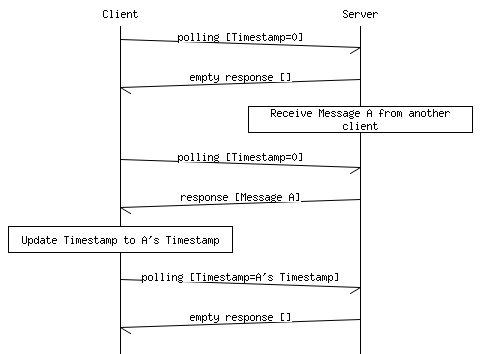
\includegraphics[width=.45\textwidth]{assets/msc/polling.png}
  \caption[Nachrichtenempfang bei Polling-Kommunikation]{Beispiel von Nachrichtenempfang bei einer klassischen Polling-Kommunikation.
    Der Client sendet regelmäßig eine Anfrage an den Server, welche entweder mit leerer Antwort oder mit neuen Inhalten beantwortet wird.
    Die Länge der Zeitspanne $\Delta t$ zwischen zwei Polling-Anfragen ist implementierungsabhängig.}
  \label{fig:polling}
\end{figure}

\begin{figure}[H]
  \centering
  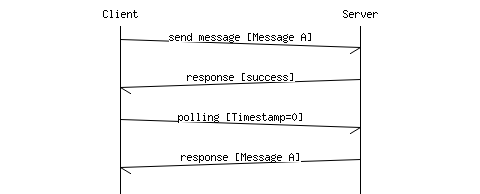
\includegraphics[width=.45\textwidth]{assets/msc/polling-send.png}
  \caption[Nachrichtenversand bei Polling-Kommunikation]{Beispiel von Nachrichtenversand bei einer klassischen Polling-Kommunikation.
    Der Client sendet eine Nachricht an den Server, welche daraufhin mittels polling abgerufen werden kann.}
  \label{fig:polling_send}
\end{figure}

Das Hauptproblem mit Polling ist der entstehende Header Overhead, der für den gesamten Zeitraum in den regelmäßigen Abfragen besteht.
Dadurch entsteht eine Netzwerkbelastung, welche keine tatsächlichen Informationen übermittelt.
In der in späteren Abschnitten vorgestellten Chatanwendung handelt es sich so zum Beispiel um 156 Bytes, die sekündlich vom Server übermittelt werden,
aber lediglich ein leeres JSON-Array enthalten.


\subsubsection{Spezifikation}
\label{sec:polling-spec}

Polling ist in der Spezifikation von HTTP nicht definiert, es handelt sich hierbei um eine Implementierung des Clients und des Servers.
Meist wird Polling durch JavaScript-Code realisiert, welcher in einem bestimmten Intervall (z. B. alle 5 Sekunden) eine Anfrage an den Server sendet.
Diese Anfrage ist ein GET-Request, welcher die URL der Anwendung enthält.
Wie der Server auf diese Anfrage antwortet, ist Implementierungsabhängig:
So könnte er zum Beispiel den gesamten abgefragten Inhalt bei jeder Anfrage übermitteln, oder nur Änderungen, die dieser Client noch nicht übermittelt bekommen hat.
Eine solche Optimierung setzt allerdings voraus, dass der Server in der Lage ist, zu identifizieren, welche Änderungen der Client bereits erhalten hat.

\subsection{Long Polling}

Eine Optimierung des Polling-Konzepts ist das sog. \emph{Long Polling}.
Dabei wird die Antwort auf eine HTTP-Anfrage zurückgehalten, bis der Server eine Nachricht versenden will \cite{noauthor_long_2021}.

\begin{figure}[H]
  \centering
  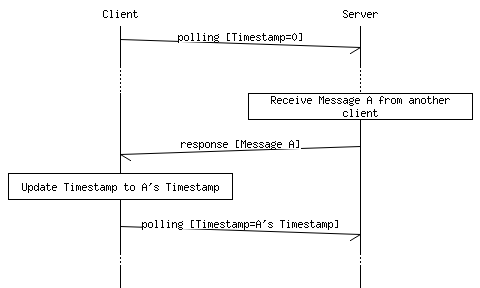
\includegraphics[width=.45\textwidth]{assets/msc/long-polling.png}
  \caption[Nachrichtenempfang bei Long Polling]{Beispiel von Nachrichtenempfang bei Long Polling.
    Der Server beantwortet die Anfrage des Clients erst, wenn er eine Nachricht hat, die er übermitteln möchte.
    Der Nachrichtenversand verläuft analog zu Polling.}
  \label{fig:long_polling}
\end{figure}

Probleme von Long Polling sind unter anderem der (im Vergleich zu klassischem Polling reduzierter, aber weiterhin präsenter)
Header Overhead, mögliche Timeouts und Ressourcen, die in Vorbereitung auf eine eingehende Nachricht vom Betriebssystem
zu Verfügung gestellt werden. \cite[Abs. 2.2]{saint-andre_known_2011}.

\subsection{Streaming}

Eine weitere Optimierung des Polling-Konzepts ist das sog. \emph{Streaming},
welches die HTTP Transferkodierung Chunking (vgl. \cite[Abs. 7.1]{fielding_http_2022}) verwendet,
also dem Aufspalten der Antwort in mehrere Packets, in welchen dann einzelne Nachrichten versendet werden.
So kann die Anzahl an Anfragen ausgehend vom Client an den Server auf eine reduziert werden --
der Server terminiert nie die Antwort auf die erste Anfrage \cite[Abs. 3]{saint-andre_known_2011}.

\begin{figure}[H]
  \centering
  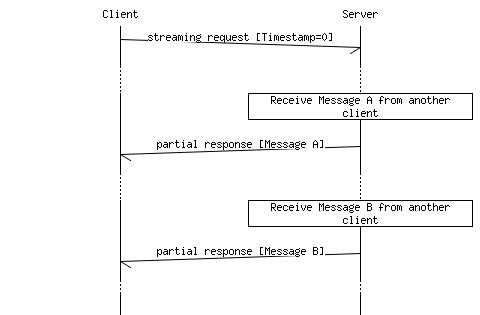
\includegraphics[width=.45\textwidth]{assets/msc/streaming.png}
  \caption[Nachrichtenempfang bei Streaming]{Beispiel von Nachrichtenempfang bei Streaming.
    Der Client initiiert den Streaming-Prozess durch eine einmalige Anfrage.
    Daraufhin sendet der Server Teilantworten an den Client, sobald neue Nachrichten verfügbar sind.
    Der Nachrichtenversand verläuft analog zu Polling.}
  \label{fig:streaming}
\end{figure}

Mit Streaming werden einige Nachteile von Polling beglichen, andere -- insb. mögliche Timeouts und unnötig reservierte Ressourcen -- bleiben bestehen.
Zusätzlich besteht das Risiko, dass diese Form von Kommunikation nicht auf allen Systemen funktioniert --
Proxys können Pakete bündeln und erst verzögert weiterleiten, wodurch Pakete ggf. nicht zeitgetreu, gebündelt oder aufgespalten ankommen \cite[Abs. 3.2]{saint-andre_known_2011}.

\subsection{WebSockets}

WebSockets sind ein vom IETF\footnote{Internet Engineering Task Force.} entwickeltes Protokoll,
welches 2011 als Standard veröffentlicht wurde \cite{melnikov_websocket_2011}.
Grund für dessen Entstehung ist unter anderem die Erkenntnis, dass der Versuch, HTTP zu verwenden,
um bidirektionale Kommunikation zu ermöglichen, vermeidbare Komplexität und Ineffizienz mit sich bringt \cite[S. 137f]{lubbers_pro_2010}.
Es ist anzumerken, dass die vorgestellten Polling-Varianten das HTTP-Protokoll effektiv missbrauchen,
um serverseitige Kommunikation zu ermöglichen:

\begin{itemize}
  \item Polling beinhaltet das Versenden von redundanten Anfragen, welche ohne Inhalt beantwortet werden,
  \item Long Polling simuliert eine Verbindung mit (sehr) hoher Latenz um eine Antwort herauszuzögern und
  \item Streaming verwendet HTTP Chunking, um innerhalb einer Response alleinstehende Nachrichten zu senden.
\end{itemize}

Die Auswirkungen dieses Missbrauchs werden auch aus der Implementierung deutlich (vgl. \autoref{sec:analysis-of-implementations}).

Diesen Missbrauch haben WebSockets nicht -- es handelt sich hierbei um ein komplett neues Protokoll,
welches diese Problemstellung direkt adressiert (vgl. \cite[Abs. 1.1]{melnikov_websocket_2011}),
indem es eine TCP-Verbindung zwischen Client und Server aufbaut und unterstützt.
Genauer baut WebSockets einen Tunnel zwischen TCP und IP auf, sodass darauffolgend TCP-Kommunikation systemübergreifend erfolgen kann (vgl. \cite[Abs. 1.5]{melnikov_websocket_2011}).
HTTP wird dann lediglich für die initialen Handshakes verwendet -- danach nicht mehr.


\begin{figure}[H]
  \centering
  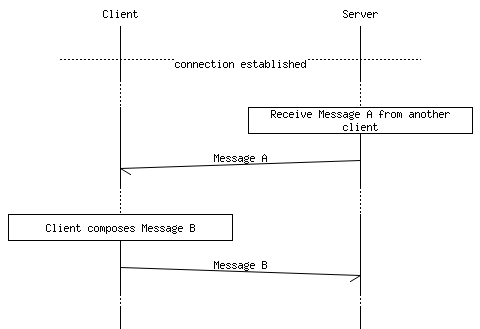
\includegraphics[width=.45\textwidth]{assets/msc/websockets.png}
  \caption[Nachrichtenaustausch bei WebSockets]{Beispiel von Nachrichtenaustausch bei WebSockets.
    Nach dem Handshake wird eine TCP-Verbindung zwischen Client und Server aufgebaut.
    Von nun an können Nachrichten in beide Richtungen ausgetauscht werden.}
  \label{fig:websockets}
\end{figure}

\subsubsection{Spezifikation}
\label{sec:websocket-spec}
Um eine Verbindung über einen WebSocker aufzubauen, wird zunächst vom Client aus eine HTTP-Anfrage gesendet.
Gemäß der Spezifikation muss es sich hierbei um eine GET-Request an den Pfad, auf dem der WebSocket hinterlegt ist, handeln.

Wäre die WebSocket URI \texttt{ws://example.org/chat}, so wäre die erste Zeile der HTTP-Anfrage \texttt{GET /chat HTTP/1.1} \cite[Abs. 4.1]{melnikov_websocket_2011}.
Zusätzlich müssen in der Anfrage unter anderem der Host (hier \texttt{Host: example.org}) und die Intention (Felder \texttt{Connection: Upgrade} und \texttt{Upgrade: websocket}) als Headerfelder übermittelt werden.

Der Server antwortet auf diese Anfrage mit einer HTTP-Response, welche entweder den Statuscode 101 \emph{Switching Protocols} oder einen Fehlercode enthält.
Zudem meldet er bei erfolgreichem Protokollwechsel die vom Client angegebene Intention zurück.

Wurde die Verbindung vom Server akzeptiert, können nun Client und Server direkt miteinander kommunizieren.
Für die Datenübermittlung sieht das WebSocket Protokoll eine auch in anderen Protokollen ähnlich vertretenes Frame-System vor,
also dem Versenden von Daten in Form von Frames, welche jeweils einen Header und eine Payload enthalten.
Header enthalten u. A. den Opcode\footnote{Opcodes (\emph{Operation Codes}, dt. \emph{Befehlscode}) können bei WebSockets Frames mit Text- oder Binärdaten ankündigen, eine vorherige Frame fortsetzen, die Verbindung schließen, oder einen Ping/Pong markieren.} und die Payload-Länge (vgl. \cite[Abs. 5.2]{melnikov_websocket_2011}).


\section{Beispielhafte Implementierungen}

Um die Unterschiede zwischen den Kommunikationsvarianten ersichtlich zu machen, werden diese für eine Chat-Applikation implementiert.
Dabei wird jeweils auf die Client- und Serverseitige Implementierung eingegangen.

Die Realisierung erfolgt in TypeScript, wobei die Serverseitige Implementierung auf Node.js basiert.
Der Client benutzt das Vue.js-Framework mit Vuetify, um die Darstellung zu vereinfachen.
Implementierungen in anderen Frontend-Frameworks erfolgen analog.
Es wird nicht auf die Darstellung der Nachrichten oder des Chats eingegangen, da dies nicht relevant für die Implementierung ist.
Entsprechende Codeabschnitte sind daher ausgelassen.

Die vollständige Implementierung der Frontendkomponenten ist im Repository im Verzeichnis \cite[\\\texttt{code/client/src/components/}]{wagner_seminar2022_2022} zu finden.
Der gesamte Code für alle Serverkomponenten befindet sich in \cite[\\\texttt{code/server/chatserver.ts}]{wagner_seminar2022_2022}.

\subsection{Implementierung von Polling}

Für alle Arten von Polling verwaltet der Server eine Liste aller bisher empfangenen Nachrichten.
Neue von einem Client übermittelte Nachrichten werden mit Autor, Zeitstempel und Text in diese Liste eingefügt.

\begin{lstlisting}[caption={Beispielhafte \emph{Message}}, label={lst:message-json}, numbers=none]
{
  content: "Hello World!",
  sender: "Alice",
  timestamp: "2022-12-04T19:29:13.455Z"
}
\end{lstlisting}

Im Falle des klassischen Polling wird der Client in regelmäßigen Zeitabständen (hier $\Delta t = 2s$) eine Anfrage an den Server senden, um neue Nachrichten abzufragen.
Dementsprechend muss der Server seine Nachrichtenliste nach für den Client neuen Nachrichten filtern und diese zurückgeben.

\subsubsection{Polling Server}

Der Server besteht aus einer Instanz von \texttt{http.Server}, welche die HTTP-Anfragen \texttt{/polling} und \texttt{/polling/send} verarbeitet.
Zudem verwaltet er ein Array mit allen Nachrichten, die bisher gesendet wurden.

Bei einer Anfrage an \texttt{/polling} wird mit einem Zeitstempel gearbeitet,
sodass der Server nur die Nachrichten zurückgibt, die nach diesem Zeitstempel eingegangen sind.

\lstinputlisting[caption={Polling Server: Nachrichtenabfrage}, label={lst:polling-server-polling}, firstlineandnumber=37, lastline=42]{../code/server/chatserver.ts}

Im Falle einer Anfrage an \texttt{/polling/send} wird die Nachricht in das Array eingefügt und der Client mit dem Statuscode 200 \emph{OK} bestätigt.

\lstinputlisting[caption={Polling Server: Nachrichtenempfang}, label={lst:polling-server-send-message}, firstlineandnumber=43, lastline=47]{../code/server/chatserver.ts}

\subsubsection{Polling Client}

Der Client besteht aus der Komponente \texttt{PollingChat.vue}, welche die Funktionen zum Senden und Empfangen von Nachrichten enthält.
Die Darstellung, sowie die Speicherung von Nachrichten und Nutzdaten erfolgt in der Komponente \texttt{ChatPage.vue} (vgl. jeweils \cite[\texttt{code/client/src/components/}]{wagner_seminar2022_2022}).

Um eine Nachricht zu versenden, wird lediglich eine HTTP POST-Anfrage an die URL \texttt{/polling/send} gesendet.
Die Nachricht wird dabei als JSON-Objekt in der Anfrage übermittelt.

\lstinputlisting[caption={Polling Client: Nachrichtenversand}, label={lst:polling-client-send-messages}, firstlineandnumber=14, lastline=22]{../code/client/src/components/PollingChat.vue}

Mittels einer HTTP POST-Anfrage an die URL \texttt{/polling} werden die Nachrichten abgefragt\footnote{Hier unterscheidet sich die Implementierung von der Spezifikation in \autoref{sec:polling-spec}. Der Zeitstempel hätte ebenfalls als Parameter übermittelt werden können.}.
Die Anfrage enthält dabei den Zeitstempel der letzten Nachricht, die der Client erhalten hat, als String.
Der Server antwortet mit einer Liste von Nachrichten, die nach diesem Zeitstempel eingegangen sind.
Diese werden anschließend an die Komponente \texttt{ChatPage.vue} mittels des Events \texttt{appendMessages} übermittelt.

Um die Nachrichten regelmäßig abzufragen, wird ein Intervall gesetzt, welches alle zwei Sekunden die Funktion \texttt{fetchMessages} aufruft.
Dieses Intervall wird bei der Initialisierung der Komponente gesetzt und bei der Entfernung der Komponente wieder gelöscht.

\lstinputlisting[caption={Polling Client: Nachrichtenabfrage}, label={lst:polling-client-get-messages}, firstlineandnumber=24, lastline=44]{../code/client/src/components/PollingChat.vue}

\subsection{Implementierung von Long Polling}

Die Implementierung von Long Polling ist sehr ähnlich zu der von Polling.
Die einzige Änderung ist, dass der Server die Anfrage nicht sofort beendet, sondern die Verbindung offen hält, bis eine neue Nachricht eingegangen ist.
Dazu wird sowohl der Client als auch der Server angepasst.

\subsubsection{Long Polling Server}

Der Server verwaltet nun eine Menge von offenen Verbindungen.
Geht eine Anfrage ein, wird diese entweder mit neuen Nachrichten beantwortet, oder die Verbindung wird in die Menge der offenen Verbindungen aufgenommen.

\lstinputlisting[caption={Long Polling Server: Nachrichtenabfrage}, label={lst:long-polling-server-get-messages}, firstlineandnumber=67, lastline=76]{../code/server/chatserver.ts}

Geht eine neue Nachricht ein, wird diese an alle bis dahin erhaltenen offenen Verbindungen gesendet.
Dadurch werden alle offenen Verbindungen geschlossen.

Aufgrund von asynchroner Bearbeitung der Anfragen kann es hier zu Race-Conditions kommen.
Daher wird der Versuch, Nachrichten an gespeicherte Verbindungen zu versenden, in einem try-catch-Block abgefangen und Errors ignoriert.

\lstinputlisting[caption={Long Polling Server: Nachrichtenempfang}, label={lst:long-polling-server-send-messages}, firstlineandnumber=77, lastline=94]{../code/server/chatserver.ts}

\subsubsection{Long Polling Client}

Der Client ändert sich ebenfalls nur minimal.
Das Versenden von Nachrichten bleibt unverändert, siehe \autoref{lst:polling-client-send-messages}.

\lstinputlisting[caption={Long Polling Client: Nachrichtenabfrage}, label={lst:long-polling-client-get-messages}, firstlineandnumber=25, lastline=41]{../code/client/src/components/LongPollingChat.vue}

\subsection{Implementierung von Streaming}

Die Implementierung von Streaming hat wieder große Ähnlichkeiten mit den vorherigen Implementierungen.

\subsubsection{Streaming Server}

Wie bei Long Polling wird auch beim Streaming eine Menge von offenen Verbindungen verwaltet.
Der Server schließt diese Verbindungen jedoch nicht mit der ersten eingehenden Nachricht, sondern lässt sie offen.

\lstinputlisting[caption={Streaming Server: Nachrichtenabfrage}, label={lst:streaming-server-get-messages}, firstlineandnumber=116, lastline=127]{../code/server/chatserver.ts}

Geht eine neue Nachricht ein, wird diese an alle gespeicherten Verbindungen gesendet.

\lstinputlisting[caption={Streaming Server: Nachrichtenempfang}, label={lst:streaming-server-send-messages}, firstlineandnumber=128, lastline=137]{../code/server/chatserver.ts}

\subsubsection{Streaming Client}

Der Client ändert sich nur minimal.
Das Versenden von Nachrichten bleibt unverändert, siehe \autoref{lst:polling-client-send-messages}.

\lstinputlisting[caption={Streaming Client: Nachrichtenabfrage}, label={lst:streaming-client-get-messages}, firstlineandnumber=23, lastline=49]{../code/client/src/components/StreamingChat.vue}

\subsection{Implementierung von WebSockets}

Da WebSockets eine vollwertige bidirektionale Kommunikation zwischen Client und Server ermöglichen, ist die Implementierung sehr einfach.

\subsubsection{WebSocket Server}

Der Server wird durch die Bibliothek \texttt{ws} unterstützt.
Diese stellt eine Klasse \texttt{WebSocket.Server} bereit, welche die Verwaltung von offenen Verbindungen übernimmt.
In dieser Implementierung erhält auch der Client, welcher die Nachricht versendet, eine Kopie der Nachricht.

\lstinputlisting[caption={WebSocket Server}, label={lst:websocket-server}, firstlineandnumber=150, lastline=163]{../code/server/chatserver.ts}

\subsubsection{WebSocket Client}

Der Client erzeugt eine \\\texttt{WebSocket} Instanz, welche die Verbindung zum Server herstellt.
Die Nachrichten werden über dessen Methode \texttt{send} versendet.
Im Falle einer neuen Nachricht wird die Callback-Funktion \texttt{onmessage} aufgerufen.

\lstinputlisting[caption={WebSocket Client}, label={lst:websocket-client}, firstlineandnumber=12, lastline=30]{../code/client/src/components/WebSocketChat.vue}

\section{Vergleiche zwischen Kommunikationsvarianten}

\subsection{Analyse der Implementierungen}
\label{sec:analysis-of-implementations}

Vergleichen wir zunächst die Implementierungen in Bezug auf Codezeilen.
Dabei wird für den Client jeweils nur der Code innerhalb des \texttt{<script>} Tags betrachtet.
Kommentar- und Leerzeilen werden nicht mitgezählt.
Es ist zudem anzumerken, dass die Zeilenanzahl nicht ausschlaggebend für die Performance ist und lediglich einen groben Überblick über den Implementierungsaufwand geben soll.

\begin{table}[h]
  \centering
  \begin{tabular}{|l|l|l|l|l|}
    \hline
    \textbf{Kommunikationsart} & \textbf{Server} & \textbf{Client} & \textbf{Gesamt} \\ \hline
    Polling                    & 23              & 31              & 54              \\
    Long Polling               & 38              & 33              & 71              \\
    Streaming                  & 31              & 37              & 68              \\
    WebSocket                  & 11              & 23              & 34              \\ \hline
  \end{tabular}
  \caption[Codezeilen pro Implementierung]{Codezeilen pro Implementierung aus \cite{wagner_seminar2022_2022}}
  \label{tab:code-lines}
\end{table}

Es ist zu erkennen, dass WebSockets wesentlich weniger Code benötigen, um das gleiche Ziel zu erreichen.
Auch ist ersichtlich, dass die Implementierung von Polling im Vergleich zu Long Polling und Streaming einfacher ist.

\subsection{Analyse der Performance}

Um die Performance der Implementierungen zu analysieren, werden zunächst Größen von Nachrichten, HTTP-Anfragen, Websocket-Verbindungen und Websocket-Nachrichten betrachtet.
Dabei wird lediglich der HTTP-Overhead betrachtet, da der TCP/UDP-Overhead nicht von der Implementierung beeinflusst werden kann.
In \autoref{tab:data-traffic-comparison} werden die übertragenen Bytemengen für die verschiedenen Implementierungen dann verglichen\footnote{Aufgrund des begrenzten Umfangs der Ausarbeitung können nicht auf Unterschiede in Latenz eingegangen werden.
  Oft ist jedoch ersichtlich, wie das Verhalten der Datenübermittlung die zeitliche Effizienz der Kommunikation beeinflusst.
  Siehe auch die Ausarbeitung von Pimentel und Nickerson, in welcher Latenzvergleiche zwischen WebSocket, Polling und Long Polling vorgenommen werden \cite{pimentel_communicating_2012}.}.
Es folgt die Berechnung der dort angegebenen Werte.

\begin{table*}[t]
  \centering
  \caption[Vergleich von übertragenen Datenmengen]{Vergleich von übertragenen Datenmengen der Implementierungen aus \cite{wagner_seminar2022_2022}}
  \label{tab:data-traffic-comparison}
  \begin{tabular}{|l|l|l|l|l|}
    \hline
    \textbf{Kommunikationsart} & \textbf{Initial} & \textbf{Regelmäßig} & \textbf{Nachrichtenempfang} & \textbf{Nachrichtenversand} \\ \hline
    Polling                    & 0 Bytes          & 771 Bytes$^a$       & 769 + $M$ Bytes             & 714 + $m$ Bytes             \\
    Long Polling               & 0 Bytes          & 0 Bytes             & 769 + $M$ Bytes             & 714 + $m$ Bytes             \\
    Streaming                  & 769 Bytes$^b$    & 0 Bytes             & $m$ Bytes                   & 714 + $m$ Bytes             \\
    WebSocket                  & 722 Bytes        & 0 Bytes             & 26 + $m$ Bytes              & 26 + $m$ Bytes              \\ \hline
  \end{tabular}\newline
  \footnotesize{$^a$ 769 Bytes gemäß \autoref{sec:message-request-size}, plus 2 für ein leeres Array als Payload.
    \\$^b$ Tatsächlich nur der Request-Teil einer Nachrichtenanfrage. Der Response-Teil wird bei der ersten eingehenden Nachricht gesendet.}
\end{table*}

\subsubsection{Größe einer \emph{Message} $m$}
Die Größe einer Nachricht (wie in \autoref{lst:message-json} dargestellt) beträgt 65 (hier sind Timestamp und JSON-Syntax enthalten) + Name + Inhalt Bytes.
Es wird in vielen Fällen ein Array von Nachrichten $M$ übertragen, wodurch sich die Größe um zwei Bytes (für die eckigen Klammern) erhöht.

\subsubsection{Größe einer Nachrichtenanfrage}
\label{sec:message-request-size}

Es handelt sich bei der Nachrichtenanfrage um eine HTTP-Anfrage vom Typ POST mit einem Payload, welches den Timestamp der letzten empfangenen Nachricht enthält.
Die Größe der Request Header der Anfrage ist stark abhängig von vielen Faktoren wie Host, Pfad, User-Agent, etc.,
weshalb hier nur mit einem ungefähren Wert von 600 Bytes gerechnet werden kann\footnote{Hier wurden die Zeichen von Request-Headern gezählt und gemittelt.
  Wird die Chat-Applikation auf localhost bereitgestellt und von einem Chrome-Browser abgerufen, beträgt der Request Header für eine Polling-Anfrage 588 Bytes.}.
Die Request-Payload ist bei Polling-Varianten ein Timestamp, welcher 24 Bytes benötigt.
Damit kommen wir auf eine Gesamtgröße von 624 Bytes für den Request-Teil der Anfrage.

Die Größe der Response ist abhängig von der Anzahl der Nachrichten, welche der Server an den Client sendet.
Der Response Header ist in der Regel 145 Bytes groß\footnote{Dieser Wert ist weniger variabel als der Request-Header,
  da hier lediglich der Status-Code, Datum und Content-Type neben ein paar HTTP-Basisdaten enthalten sind.}.
Ist die Antwort leer, so ist die Größe der Response-Payload 2 Bytes (für ein leeres Array).
Damit kommen wir auf eine Gesamtgröße von 147 Bytes für den Response-Teil der Anfrage.

Anfragen mit einer leeren Antwort haben eine Gesamtgröße von 771 Bytes.
Anfragen mit einer Antwort, welche Nachrichten enthält, haben eine Gesamtgröße von 769 + $M$ Bytes.

\subsubsection{Größe einer Nachrichtenübermittlung}
Der Request Header bleibt gleich, da die Nachrichtenübermittlung ebenfalls über eine POST-Request erfolgt.
Die Größe der Request-Payload ist 65 Bytes + Name + Inhalt Bytes.

Die Response hat eine Größe von 114 Bytes – hier enthält der Response-Header nur den Status-Code und das Datum, da keine Payload übertragen wird.

Damit kommen wir auf eine Gesamtgröße von 714 + $m$ Bytes für eine Nachrichtenübermittlung.


\subsubsection{Größe eines Websocket-Verbindungsaufbaus}
Für den Protokollwechsel versendet der Client eine HTTP-Anfrage vom Typ GET mit einem Request-Header, welcher den Wechsel zum WebSocket-Protokoll startet (vgl. hierzu \autoref{sec:websocket-spec}).
Auch hier gehen wir bei dem Request Header von einer durchschnittlichen Größe von 600 Bytes aus.
Bei GET-Requests ist die Request-Payload leer, sodass die Gesamtgröße des Request-Teils 600 Bytes beträgt.

Die Response hat eine Größe von 122 Bytes – hier enthält der Response Header lediglich den Status-Code und die Ankündigung, dass der Protokollwechsel erfolgreich war.
Die Response-Payload ist ebenfalls leer, sodass die Gesamtgröße des Response-Teils 122 Bytes beträgt.

Der Aufbau einer Websocket-Verbindung hat somit eine Gesamtgröße von 722 Bytes.

\subsubsection{Größe einer Websocket-Nachricht}
Nachrichten, die über eine Websocket-Verbindung übertragen werden, haben keinen HTTP-Overhead.
Die Größe einer Nachricht ist daher rein die Größe der \emph{Message} $m$ plus dem WebSocket-Overhead.
Dieser gibt den Typ der WebSocket-Nachricht an und hat einen Overhead von 26 Bytes im Falle des Typs \texttt{message}.
Dies gilt sowohl für gesendete als auch empfangene Nachrichten.

Eine WebSocket-Nachricht hat somit eine Gesamtgröße von 26 + $m$ Bytes.

\subsubsection{Schlussfolgerungen}

Anhand der \autoref{tab:data-traffic-comparison} ist ersichtlich, dass die Menge an Datenverkehr abhängig von der Implementierung in unterschiedlichen Abschnitten der Kommunikation variiert.
Es ist anzumerken, dass die Größe der Nachrichten großen Einfluss auf die Größe des Datenverkehrs darstellt.
Polling ist die einzige Variante, bei der ein regelmäßiger Datenverkehr entsteht.
Wie oft die Anfragen versendet werden, ist abhängig von der Implementierung bzw. dem gewählten Polling-Intervall $\Delta t$.

Es lässt sich argumentieren, dass die klassische Polling-Variante attraktiver als Long Polling und Streaming ist, wenn über einen kleinen Zeitraum viele Nachrichten übertragen werden sollen, da hier dann weniger Datenverkehr entsteht.
Bei einer längeren Zeit, in der keine Nachrichten übertragen werden, ist die klassische Polling-Variante jedoch weniger attraktiv, da hier redundanter Datenverkehr entsteht.
Auch könnte dieser Vorteil bei Long Polling und Streaming genutzt werden, indem die Anfragen nur alle $\Delta t$ Sekunden beantwortet werden.

Für eine Echtzeitkommunikation kommen alle Kommunikationsvarianten bis auf Polling infrage, da in allen anderen Fällen die Nachrichten sofort übertragen werden.
Kommen viele Nachrichten schnell aufeinander, kann es passieren, dass Long Polling mehrere Nachrichten in einem Request versendet, da es immer auf eine neue Anfrage warten muss.
In diesem Fall wäre Streaming die bessere Wahl, da hier die Nachrichten sofort übertragen werden können.

Generell ist Streaming Long Polling vorzuziehen, da es den Overhead für Nachrichtenempfang reduziert, indem es Redundanzen vermeidet.

WebSockets sind bei weitem die an Overhead geringste Variante, da hier keine HTTP-Requests und -Responses benötigt werden.
Da hier eine TCP-Verbindung aufgebaut wird, ist die Nachrichtenübertragung wesentlich effizienter.

\subsection{Auswahl einer Kommunikationsvariante für die Chatanwendung}

Für den Anwendungsfall der Chatanwendung ist die Wahl der Kommunikationsvariante abhängig von der Anzahl und Art der Nutzer sowie der Anzahl der Nachrichten, die übertragen werden sollen.
WebSockets sind ein relativ neues Feature und werden von älteren Browsern nicht unterstützt.
Bei den meisten Browsern wurden WebSockets in Versionen von etwa 2012 implementiert \cite{deveria_web_nodate}.
Soll die Chatanwendung auf möglichst vielen Browsern laufen, ist es sinnvoll, eine Kommunikationsvariante zu wählen, die auch von älteren Browsern unterstützt wird.
Dabei ist anzumerken, dass der geschätzte Anteil der Nutzer, die einen Browser mit WebSocket-Fähigkeit verwenden, auf etwa $98.3\%$ geschätzt wird \cite{deveria_web_nodate}.
So bildet der Anteil an Nutzern, die keine WebSocket-Verbindungen aufbauen können, eine eventuell vernachlässigbare Minderheit.

Die Wahl für die Chatanwendung fällt eindeutig auf WebSockets, da diese die geringste Latenz aufweisen \cite{pimentel_communicating_2012} und die Nachrichten mit minimalem Overhead übertragen werden können.
Auch ist davon auszugehen, dass die meisten Nutzer der Chatanwendung einen Browser mit WebSocket-Fähigkeit verwenden werden.

\subsubsection{Auswahl mit Priorität auf Verfügbarkeit}

Muss die Chatanwendung auf fast allen Browsern laufen, darf WebSockets nicht verwendet werden.
Nun muss entschieden werden, welche der anderen Kommunikationsvarianten sinnvoll ist.

Werden sehr viele Nachrichten von vielen Nutzern gleichzeitig versendet, kommen Streaming oder Polling infrage:
Streaming, da hier die Nachrichten mit minimalem Overhead sofort übertragen werden können; und
Polling, da Mengen von Nachrichten in regelmäßigen Abständen übertragen werden können.
Hierbei ist anzumerken, dass Polling eine hohe Netzwerkbelastung verursachen kann, wenn viele Nutzer die Nachrichten gleichzeitig abfragen.
So würden 1.000 Nutzer, die sekündlich Nachrichten anfragen, allein durch die Header etwa 6 Mbps an Netzwerkdurchsatz verursachen \cite{lubbers_html5_nodate}.

Dann kann je nach Priorität – Effizienz bei großen Mengen von Nachrichten oder Echtzeit – entschieden werden, welche Variante verwendet werden soll.
Werden in der Regel nur wenige Nachrichten versendet, ist Streaming die beste Wahl, da es den geringsten Overhead mit Echtzeitübermittlung hat.


\section{Vorstellung von Frameworks}

Es gibt Frameworks, die das Implementieren von asynchroner Kommunikation erleichtern.

\subsection{Socket.IO}

Was ist das? Wie ist es besser oder schlechter für die Implementierung als Chat-App? Performance?
Auch: Attraktiv für Verfügbarkeit, da es auf allen Browsern läuft. Weicht auf Polling aus, wenn WebSockets nicht unterstützt werden.

\subsection{Faye}

\section{Fazit}


\bibliographystyle{literature/bibtex/IEEEtran}
\bibliography{literature/literature}

\listoffigures
\listoftables

\end{document}}